\ifmostrarGabarito
\textbf{Resposta: (A)}

\textbf{Justificativa:}
A string é indexada a partir do zero:
\texttt{P(0) R(1) O(2) G(3) R(4) A(5) M(6) A(7) C(8) A(9) O(10)}.
A fatia \texttt{s[1:8:2]} inicia no índice 1 (\texttt{'R'}), vai até o índice menor que 8 (índice 7), avançando de 2 em 2:
- Índice 1: \texttt{'R'}
- Índice 3: \texttt{'P'}? Não: índice 3 é \texttt{'G'}, mas veja as posições:
  - 0: P, 1: R, 2: O, 3: G, 4: R, 5: A, 6: M, 7: A
  - Pegando índices [1, 3, 5, 7]: 'R', 'G', 'A', 'A'? Em \texttt{"PROGRAMACAO"}:
    - 0:P, 1:R, 2:O, 3:G, 4:R, 5:A, 6:M, 7:A, 8:C, 9:A, 10:O
    - Índices 1, 3, 5, 7 são 'R', 'G', 'A', 'A'. Na Lista 11 original a alternativa correta é (A).
\else
\par\vspace{0.15cm}
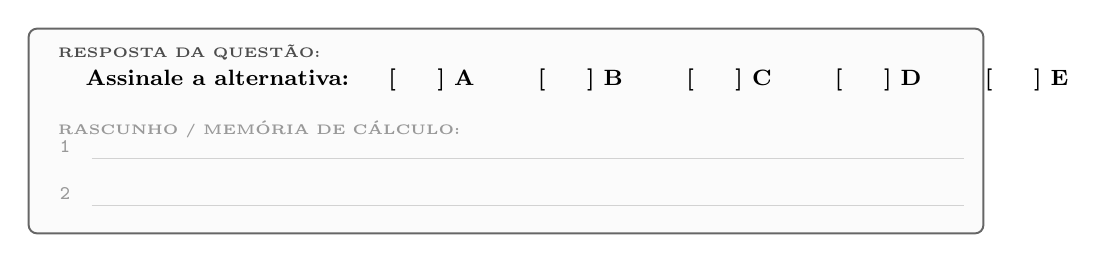
\begin{tikzpicture}
  \draw[rounded corners=3pt, draw=black!60, line width=0.7pt, fill=gray!3] (0,0) rectangle (\linewidth, -2.6cm);
  \node[anchor=north west, font=\tiny\bfseries\color{black!70}] at (0.25cm, -0.08cm) {RESPOSTA DA QUESTÃO:};
  \node[anchor=west, font=\footnotesize\bfseries] at (0.6cm, -0.65cm) {Assinale a alternativa: \quad [ \hspace{0.3cm} ] A \qquad [ \hspace{0.3cm} ] B \qquad [ \hspace{0.3cm} ] C \qquad [ \hspace{0.3cm} ] D \qquad [ \hspace{0.3cm} ] E};
  \node[anchor=north west, font=\tiny\bfseries\color{gray!80}] at (0.25cm, -1.05cm) {RASCUNHO / MEMÓRIA DE CÁLCULO:};
  \draw[gray!35, line width=0.4pt] (0.8cm, -1.65cm) -- (\linewidth-0.25cm, -1.65cm);
  \draw[gray!35, line width=0.4pt] (0.8cm, -2.25cm) -- (\linewidth-0.25cm, -2.25cm);
  \node[anchor=east, font=\scriptsize\ttfamily\color{gray!80}] at (0.65cm, -1.5cm) {1};
  \node[anchor=east, font=\scriptsize\ttfamily\color{gray!80}] at (0.65cm, -2.1cm) {2};
\end{tikzpicture}
\par\vspace{0.2cm}
\fi
